% Provenance (never printed): cycle 4 SVT/physique, "La planete Terre,
% l'environnement": the movements of the atmosphere, weather and its
% forecast; see sources/book1/PROVENANCE.md. Book 1, grade 8, chapter 3.
% Vocabulary guard: owns air mass, front (warm, cold), depression (homograph:
% phrase-level linking only), anticyclone, isobar, weather forecast. The
% rotation of the winds around lows and highs is told (deflection, recalled
% from ch. g8.2); the occluded front is named in prose only; numerical models
% are told, not taught.
\chapter{Masas de aire, frentes y mapas del tiempo}\label{ch:g8:fronts-and-weather-maps}

La mañana es luminosa y tranquila. Hacia mediodía aparecen unas finas
estrías blancas muy altas en el cielo, que se van extendiendo lentamente en
un velo pálido que atenúa el Sol. Por la tarde las \omterm{def:g4:clouds-rain-snow:cloud}{nubes} se espesan y
bajan; al anochecer cae una \omterm{def:g4:clouds-rain-snow:precipitation}{lluvia} continua. Durante la noche el aire se
vuelve templado y húmedo, y luego una línea oscura de \omterm{def:g4:clouds-rain-snow:cloud}{nubes} trae un breve
chaparrón intenso y una racha de viento. A la mañana siguiente el cielo
está despejado, el aire fresco y hace viento. En dos días ha pasado sobre la
ciudad una \emph{\omterm{def:g8:fronts-and-weather-maps:depression}{borrasca}}, con sus dos \omterm{def:g8:fronts-and-weather-maps:front}{frentes}.
% ledger: ucar:warm-front, ucar:cold-front

\begin{omfigure}
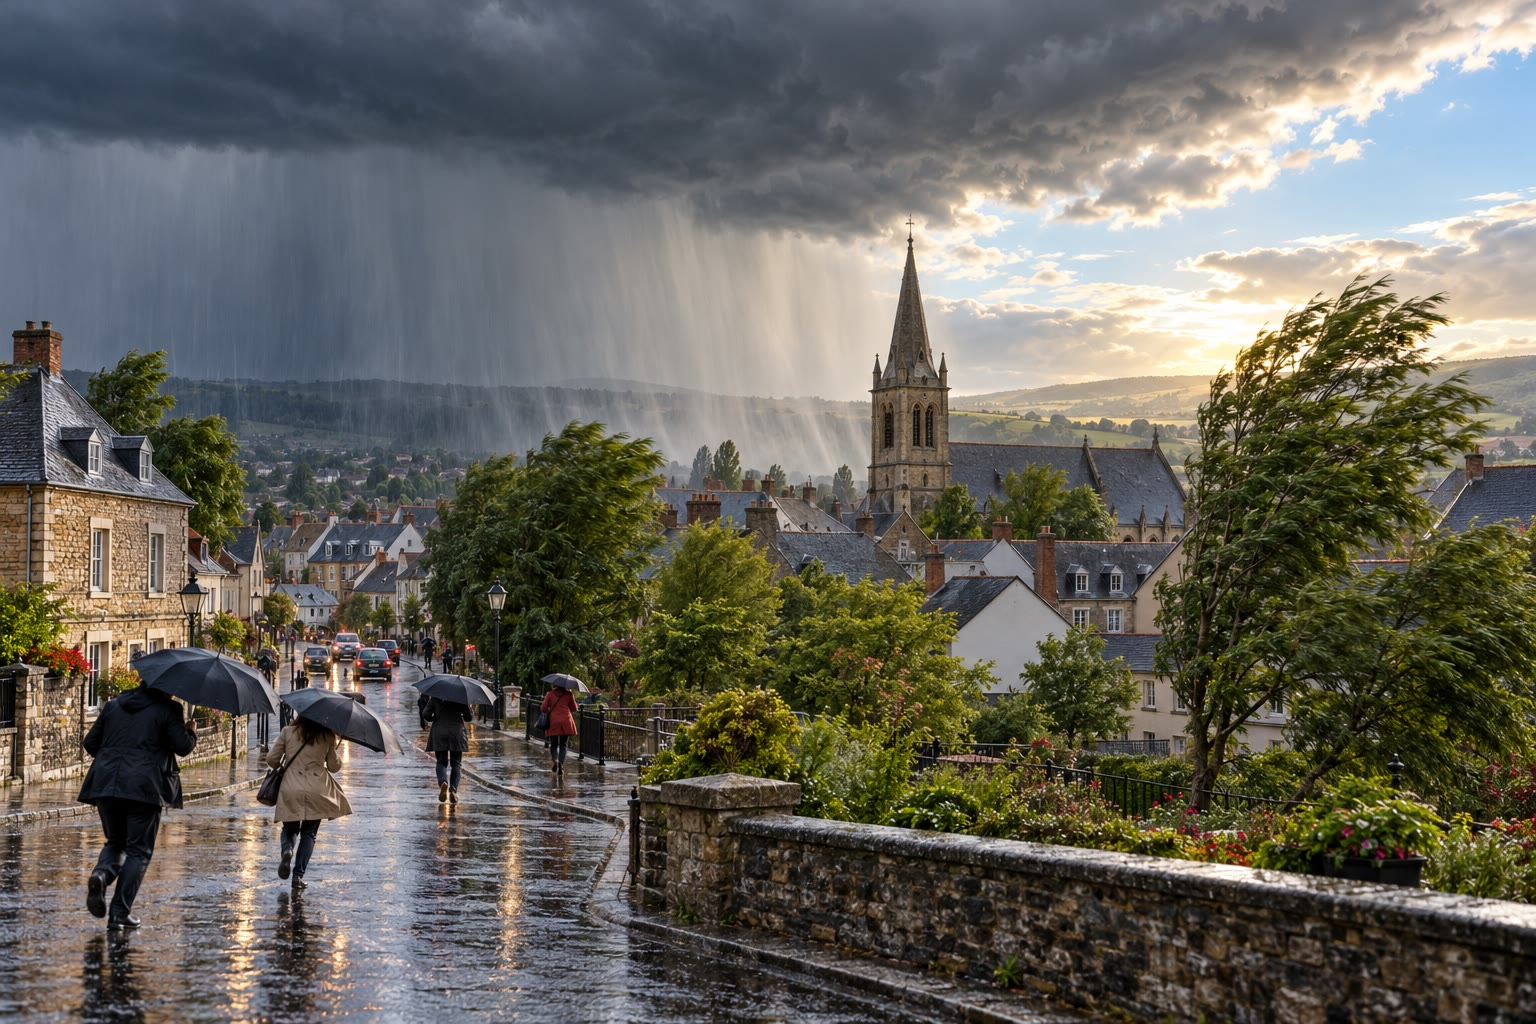
\includegraphics[width=0.6\linewidth]{images/book1/ai/g8-rain-arriving.jpg}

{\small Una cortina de \omterm{def:g4:clouds-rain-snow:precipitation}{lluvia} llega sobre una ciudad bajo una base de \omterm{def:g4:clouds-rain-snow:cloud}{nubes}
oscura, mientras el cielo sigue despejado detrás de la iglesia
(ilustración generada por IA de una escena genérica).}
\label{fig:g8:fronts-and-weather-maps:rain}
\end{omfigure}

Los meteorólogos lo vieron venir con días de antelación. Este capítulo
muestra cómo: el aire de nuestros cielos llega en grandes masas, las masas
se encuentran a lo largo de \omterm{def:g8:fronts-and-weather-maps:front}{frentes}, y los \omterm{def:g2:drawing-to-map:map}{mapas} de presión muestran
adónde se dirigen.

\begin{recall}
El aire presiona sobre todo lo que toca; un barómetro mide esa presión en
hectopascales (los libros de física), y al \omterm{def:g4:world-physical-map:altitude}{nivel del mar} es de unos
\qty{1013}{hPa} (\cref{ch:g8:the-atmosphere}). Las \omterm{def:g4:clouds-rain-snow:cloud}{nubes} se forman cuando
el aire húmedo sube y se enfría (\cref{ch:g4:clouds-rain-snow}). En el
suelo, el viento sopla de las altas presiones hacia las bajas, y la
rotación de la Tierra lo desvía: hacia la derecha en el \omterm{def:g3:continents-and-oceans:equator}{hemisferio norte}.
Entre unos \ang{30} y \ang{60}, los \omterm{def:g8:winds-global-circulation:global-winds}{vientos del oeste} traen una \omterm{def:g8:fronts-and-weather-maps:depression}{borrasca}
tras otra (\cref{ch:g8:winds-global-circulation}).
\end{recall}

\section{Las masas de aire}

El aire que permanece varios días sobre el mismo lugar adquiere el carácter
de la superficie que tiene debajo. Sobre un \omterm{def:g2:water-on-earth:ocean}{océano} cálido se vuelve cálido
y húmedo; sobre una tierra helada, frío y seco. Cuando se aleja, lleva
consigo ese carácter, a veces a lo largo de miles de kilómetros.
% ledger: noaa:air-mass

\begin{definition}[Masa de aire]\label{def:g8:fronts-and-weather-maps:air-mass}
Una \emph{masa de aire}\index{masa de aire} es un volumen de aire muy
grande en el que la temperatura y la humedad son casi las mismas en todas
partes a una altura dada. Las toma de la región donde se formó, su
\emph{región de origen}.
\end{definition}
% ledger: noaa:air-mass

Los meteorólogos designan una \omterm{def:g8:fronts-and-weather-maps:air-mass}{masa de aire} con dos letras. La primera
indica dónde se formó: \emph{c} (continental), sobre tierra firme, así que
es seca; \emph{m} (marítima), sobre un \omterm{def:g2:water-on-earth:ocean}{océano}, así que es húmeda. La
segunda indica lo fría que es: \emph{A} (ártica), sobre las regiones
polares; \emph{P} (polar), sobre las \omterm{def:g6:latitude-longitude:latitude}{latitudes} altas; \emph{T} (tropical),
sobre las \omterm{def:g6:latitude-longitude:latitude}{latitudes} bajas. El aire de un \omterm{def:g5:weather-and-climate:desert}{desierto} cálido es cT, cálido y
seco; el aire del Ártico es cA, muy frío y seco.
% ledger: noaa:air-mass

\begin{omfigure}
\begin{tikzpicture}
\begin{axis}[ommap, width=12.6cm, xmin=-100, xmax=60, ymin=10, ymax=85,
  xtick={-90,-60,...,60}, ytick={20,40,60,80},
  xticklabels={$90^\circ$O,$60^\circ$O,$30^\circ$O,$0^\circ$,$30^\circ$E,$60^\circ$E},
  yticklabels={$20^\circ$N,$40^\circ$N,$60^\circ$N,$80^\circ$N},
  tick label style={font=\scriptsize}]
  \addplot[fill=omLithAlluv, draw=black!45, line width=0.2pt] table {figdata/out/shared-geo-land.dat};
  \tikzset{src/.style={line width=0.9pt, fill opacity=0.35, text opacity=1, font=\scriptsize, align=center}}
  \draw[src, draw=omCold, fill=omCold!35] (axis cs:-30,79) ellipse [x radius=26, y radius=4.5];
  \node[font=\scriptsize, align=center, fill=white, inner sep=1pt] at (axis cs:-30,79) {\textbf{cA}: muy fría, seca};
  \draw[src, draw=omCold, fill=omCold!25] (axis cs:-35,55) ellipse [x radius=14, y radius=6];
  \node[font=\scriptsize, align=center, fill=white, inner sep=1pt] at (axis cs:-35,55) {\textbf{mP}: fría,\\ húmeda};
  \draw[src, draw=omCold, fill=omCold!25] (axis cs:-84,60) ellipse [x radius=12, y radius=7];
  \node[font=\scriptsize, align=center, fill=white, inner sep=1pt] at (axis cs:-84,60) {\textbf{cP}: fría,\\ seca};
  \draw[src, draw=omCold, fill=omCold!25] (axis cs:45,62) ellipse [x radius=14, y radius=7];
  \node[font=\scriptsize, align=center, fill=white, inner sep=1pt] at (axis cs:45,62) {\textbf{cP}: fría,\\ seca};
  \draw[src, draw=omWarm, fill=omWarm!25] (axis cs:-45,28) ellipse [x radius=16, y radius=6];
  \node[font=\scriptsize, align=center, fill=white, inner sep=1pt] at (axis cs:-45,28) {\textbf{mT}: cálida,\\ húmeda};
  \draw[src, draw=omWarm, fill=omWarm!25] (axis cs:10,24) ellipse [x radius=15, y radius=6];
  \node[font=\scriptsize, align=center, fill=white, inner sep=1pt] at (axis cs:10,24) {\textbf{cT}: muy cálida,\\ seca};
\end{axis}
\end{tikzpicture}

{\small Regiones de origen típicas de las \omterm{def:g8:fronts-and-weather-maps:air-mass}{masas de aire} en torno al
Atlántico Norte (esquema): sobre el Ártico, los \omterm{def:g3:continents-and-oceans:continent}{continentes} fríos, el
\omterm{def:g2:water-on-earth:ocean}{océano} septentrional, el \omterm{def:g2:water-on-earth:ocean}{océano} subtropical y el Sáhara. En azul: \omterm{def:g8:fronts-and-weather-maps:air-mass}{masas de
aire} frías; en rojo: masas cálidas.}
% ledger: noaa:air-mass, data:ne-land (schematic regions)
\label{fig:g8:fronts-and-weather-maps:sources}
\end{omfigure}

\section{Los frentes}

Cuando una \omterm{def:g8:fronts-and-weather-maps:air-mass}{masa de aire} se desplaza, se encuentra con otra. Las dos no se
mezclan fácilmente: se mantienen separadas, con una frontera estrecha entre
ellas donde el \omterm{def:g1:watching-the-weather:weather}{tiempo} cambia.
% ledger: mo:fronts, ucar:cold-front

\begin{definition}[Frente]\label{def:g8:fronts-and-weather-maps:front}
Un \emph{frente}\index{frente} es la frontera, en el suelo, entre dos \omterm{def:g8:fronts-and-weather-maps:air-mass}{masas
de aire} de temperatura y humedad distintas. En un
\emph{frente frío}\index{frente frio@frente frío}, el aire frío avanza
contra un aire más cálido y ocupa su lugar; en un
\emph{frente cálido}\index{frente calido@frente cálido}, el aire cálido
avanza contra un aire más frío y ocupa su lugar.
\end{definition}
% ledger: mo:fronts, ucar:cold-front, ucar:warm-front

El aire frío es más denso que el aire cálido. En un \omterm{def:g8:fronts-and-weather-maps:front}{frente frío}, el aire
frío se desliza bajo el aire cálido como una cuña y lo levanta
bruscamente. El aire cálido y húmedo sube deprisa y forma \omterm{def:g4:clouds-rain-snow:cloud}{nubes} de gran
desarrollo vertical, \omterm{def:g4:clouds-rain-snow:cloud-families}{cúmulos} y \omterm{def:g4:clouds-rain-snow:cloud-families}{cumulonimbos}: el \omterm{def:g8:fronts-and-weather-maps:front}{frente} trae chubascos
fuertes, a veces \omterm{def:g4:clouds-rain-snow:precipitation}{granizo} y truenos, rachas de viento y un descenso brusco
de la temperatura. Una vez que ha pasado, la \omterm{def:g4:clouds-rain-snow:precipitation}{lluvia} cesa y el cielo se
despeja. Un \omterm{def:g8:fronts-and-weather-maps:front}{frente frío} avanza deprisa, hasta el doble de rápido que un
\omterm{def:g8:fronts-and-weather-maps:front}{frente cálido}.
% ledger: ucar:cold-front

\begin{omfigure}
\begin{tikzpicture}[font=\footnotesize, >={Stealth[length=2.2mm]}, yscale=0.7, xscale=0.95]
  % ground
  \draw[line width=0.8pt] (0,0) -- (15,0);
  % cold wedge, nose at x = 8.2
  \fill[omCold!18] (0,0) -- (0,3.4) .. controls (4.5,3.2) and (7.2,2.4) .. (7.9,0.8)
    .. controls (8.1,0.35) and (8.2,0.12) .. (8.25,0) -- cycle;
  \draw[omCold, line width=1pt] (0,3.4) .. controls (4.5,3.2) and (7.2,2.4) .. (7.9,0.8)
    .. controls (8.1,0.35) and (8.2,0.12) .. (8.25,0);
  \node[omCold, align=center] at (3.2,1.4) {\textbf{aire frío}\\(denso)};
  \node[omWarm, align=center] at (12.6,1.4) {\textbf{aire cálido}\\\textbf{y húmedo}};
  % cold air pushes
  \draw[->, omCold, line width=1.2pt] (4.6,0.5) -- (7.0,0.5);
  % warm air lifted
  \draw[->, omWarm, line width=1.2pt] (11.2,0.45) .. controls (9.4,0.6) and (8.6,1.4) .. (8.5,3.0);
  % cumulonimbus
  \fill[black!12] (7.3,2.6) .. controls (7.0,3.4) and (7.4,4.2) .. (7.9,4.5)
    .. controls (7.6,5.0) and (8.6,5.2) .. (9.4,5.1) -- (11.0,5.15)
    .. controls (10.6,4.9) and (10.2,4.8) .. (10.0,4.6)
    .. controls (10.4,4.0) and (10.2,3.0) .. (9.8,2.5) -- cycle;
  \draw[black!45] (7.3,2.6) .. controls (7.0,3.4) and (7.4,4.2) .. (7.9,4.5)
    .. controls (7.6,5.0) and (8.6,5.2) .. (9.4,5.1) -- (11.0,5.15)
    .. controls (10.6,4.9) and (10.2,4.8) .. (10.0,4.6)
    .. controls (10.4,4.0) and (10.2,3.0) .. (9.8,2.5) -- cycle;
  \node at (9.0,3.8) {cumulonimbo};
  \foreach \x in {7.7,8.0,...,9.6} \draw[omCold!70, line width=0.5pt] (\x,2.45) -- (\x-0.25,0.15);
  \node[anchor=west, align=left] at (9.8,1.95) {chubascos fuertes,\\rachas};
  % motion
  \draw[->, line width=1.3pt] (5.7,4.3) -- (7.2,4.3);
  \node[anchor=east] at (5.6,4.3) {el frente avanza};
  \node[anchor=north] at (8.25,-0.1) {frente en el suelo};
  \node[anchor=north west, align=left] at (0.1,-0.1) {detrás: más fresco, despejando};
  \node[anchor=north east, align=right] at (15,-0.1) {delante: cálido, húmedo};
\end{tikzpicture}

{\small Un \omterm{def:g8:fronts-and-weather-maps:front}{frente frío} visto de lado (alturas muy exageradas). El aire frío
se mete bajo el aire cálido como una cuña; el aire cálido se eleva
bruscamente y forma \omterm{def:g4:clouds-rain-snow:cloud}{nubes} de gran desarrollo vertical.}
% ledger: ucar:cold-front
\label{fig:g8:fronts-and-weather-maps:cold}
\end{omfigure}

En un \omterm{def:g8:fronts-and-weather-maps:front}{frente cálido}, el aire cálido, ligero, no puede apartar del suelo al
aire frío: sube lentamente por encima de él, por una pendiente larga y
suave. Por eso sus \omterm{def:g4:clouds-rain-snow:cloud}{nubes} aparecen mucho antes de que llegue el \omterm{def:g8:fronts-and-weather-maps:front}{frente}, muy
altas en el cielo: primero finas estrías de \omterm{def:g4:clouds-rain-snow:cloud-families}{cirros}, luego un velo de
cirrostratos y después altostratos grises. A medida que el \omterm{def:g8:fronts-and-weather-maps:front}{frente} se
acerca, las \omterm{def:g4:clouds-rain-snow:cloud}{nubes} bajan y se espesan, y empieza una \omterm{def:g4:clouds-rain-snow:precipitation}{lluvia} larga y
continua. Después de que pase, el aire es más cálido y más húmedo.
% ledger: ucar:warm-front, bom:isobars (warm front: steady rain, grey skies)

\begin{omfigure}
\begin{tikzpicture}[font=\footnotesize, >={Stealth[length=2.2mm]}]
  \draw[line width=0.8pt] (0,0) -- (15,0);
  % cold air ahead (right), warm air climbing a gentle slope from the front at x = 2.2
  \fill[omCold!18] (2.2,0) .. controls (6,0.9) and (10,2.2) .. (15,3.4) -- (15,0) -- cycle;
  \draw[omCold, line width=1pt] (2.2,0) .. controls (6,0.9) and (10,2.2) .. (15,3.4);
  \node[omCold, align=center] at (11.8,0.75) {\textbf{aire frío}};
  \node[omWarm, align=center] at (1.4,1.6) {\textbf{aire cálido}\\\textbf{y húmedo}};
  \draw[->, omWarm, line width=1.2pt] (1.0,0.45) .. controls (4.5,0.9) and (8.5,2.4) .. (12.4,3.4);
  % clouds: nimbostratus near the front, altostratus, cirrostratus, cirrus far ahead
  \fill[black!18] (2.4,0.7) .. controls (3.2,1.8) and (5.5,2.3) .. (6.6,2.4) -- (6.4,1.25) .. controls (5,1.0) and (3.8,0.7) .. cycle;
  \node at (5.4,1.62) {nimbostratos};
  \foreach \x in {3.0,3.3,...,5.7} \draw[omCold!70, line width=0.5pt] (\x,0.95) -- (\x-0.2,0.25);
  \fill[black!10, rounded corners=4pt] (6.4,2.65) rectangle (10.0,3.25);
  \node at (8.2,2.95) {altostratos};
  \fill[black!6, rounded corners=4pt] (9.6,3.75) rectangle (12.6,4.15);
  \node at (11.1,3.95) {cirrostratos};
  \foreach \x in {12.6,13.2,13.8} \draw[black!35, line width=0.6pt] (\x,4.55) .. controls (\x+0.2,4.75) and (\x+0.4,4.6) .. (\x+0.55,4.85);
  \node[anchor=south] at (13.4,4.9) {cirros};
  \draw[->, line width=1.3pt] (2.6,4.3) -- (4.1,4.3);
  \node[anchor=east] at (2.5,4.3) {el frente avanza};
  \node[anchor=north] at (2.2,-0.1) {frente en el suelo};
  \node[anchor=north east] at (15,-0.1) {muy por delante: las primeras nubes altas};
\end{tikzpicture}

{\small Un \omterm{def:g8:fronts-and-weather-maps:front}{frente cálido} visto de lado (alturas muy exageradas). El aire
cálido sube lentamente por encima del aire frío; sus \omterm{def:g4:clouds-rain-snow:cloud}{nubes} bajan y se
espesan a medida que el \omterm{def:g8:fronts-and-weather-maps:front}{frente} se acerca, y la \omterm{def:g4:clouds-rain-snow:precipitation}{lluvia} es larga y continua.}
% ledger: ucar:warm-front
\label{fig:g8:fronts-and-weather-maps:warm}
\end{omfigure}

En un \omterm{def:g2:drawing-to-map:map}{mapa} del \omterm{def:g1:watching-the-weather:weather}{tiempo}, un \omterm{def:g8:fronts-and-weather-maps:front}{frente frío} se dibuja como una línea azul con
triángulos, y un \omterm{def:g8:fronts-and-weather-maps:front}{frente cálido}, como una línea roja con semicírculos. Los
símbolos están del lado hacia el que avanza el \omterm{def:g8:fronts-and-weather-maps:front}{frente}. Cuando un \omterm{def:g8:fronts-and-weather-maps:front}{frente
frío} rápido alcanza a un \omterm{def:g8:fronts-and-weather-maps:front}{frente cálido}, los dos se unen en un \emph{\omterm{def:g8:fronts-and-weather-maps:front}{frente}
ocluido}, que se dibuja en violeta con los dos símbolos.
% ledger: mo:fronts, ucar:cold-front

\section{Borrascas y anticiclones}

Los \omterm{def:g8:fronts-and-weather-maps:front}{frentes} nacen en los grandes torbellinos de aire que atraviesan las
\omterm{def:g6:latitude-longitude:latitude}{latitudes} medias. Donde el aire sube, la presión en el suelo es más baja
que en todo su alrededor; donde baja, la presión es más alta.
% ledger: bom:highs-lows

\begin{definition}[Borrasca y anticiclón]\label{def:g8:fronts-and-weather-maps:depression}
Una \emph{borrasca}\index{borrasca}, o baja, es una región donde la presión
al \omterm{def:g4:world-physical-map:altitude}{nivel del mar} es más baja que en todo su alrededor. Un
\emph{anticiclón}\index{anticiclon@anticiclón}, o alta, es una región donde
es más alta que en todo su alrededor.
\end{definition}
% ledger: bom:isobars, bom:highs-lows
\phantomsection\label{def:g8:fronts-and-weather-maps:anticyclone}

El viento sopla de la alta hacia la baja, pero la rotación de la Tierra lo
desvía, así que acaba soplando casi alrededor de los centros. En el
\omterm{def:g3:continents-and-oceans:equator}{hemisferio norte} gira en sentido contrario a las agujas del reloj alrededor
de una \omterm{def:g8:fronts-and-weather-maps:depression}{borrasca}, y en el sentido de las agujas del reloj alrededor de un
\omterm{def:g8:fronts-and-weather-maps:depression}{anticiclón}; en el \omterm{def:g3:continents-and-oceans:equator}{hemisferio sur}, al revés. En una \omterm{def:g8:fronts-and-weather-maps:depression}{borrasca}, el aire
converge cerca del suelo, sube, se enfría y forma \omterm{def:g4:clouds-rain-snow:cloud}{nubes}: las \omterm{def:g8:fronts-and-weather-maps:depression}{borrascas}
traen \omterm{def:g4:clouds-rain-snow:cloud}{nubes}, \omterm{def:g4:clouds-rain-snow:precipitation}{lluvia} y viento, y sus \omterm{def:g8:fronts-and-weather-maps:front}{frentes}. En un \omterm{def:g8:fronts-and-weather-maps:depression}{anticiclón}, el aire
baja y se calienta al descender: los \omterm{def:g8:fronts-and-weather-maps:depression}{anticiclones} traen un \omterm{def:g1:watching-the-weather:weather}{tiempo} seco y
estable, con vientos flojos. Un \omterm{def:g8:fronts-and-weather-maps:depression}{anticiclón} típico tiene una presión de unos
\qty{1020}{hPa} o más en su centro; una \omterm{def:g8:fronts-and-weather-maps:depression}{borrasca} profunda baja de
\qty{980}{hPa}.
% ledger: bom:highs-lows, bom:isobars, mo:global-circ

\begin{omfigure}
\begin{minipage}[c]{0.36\linewidth}\centering
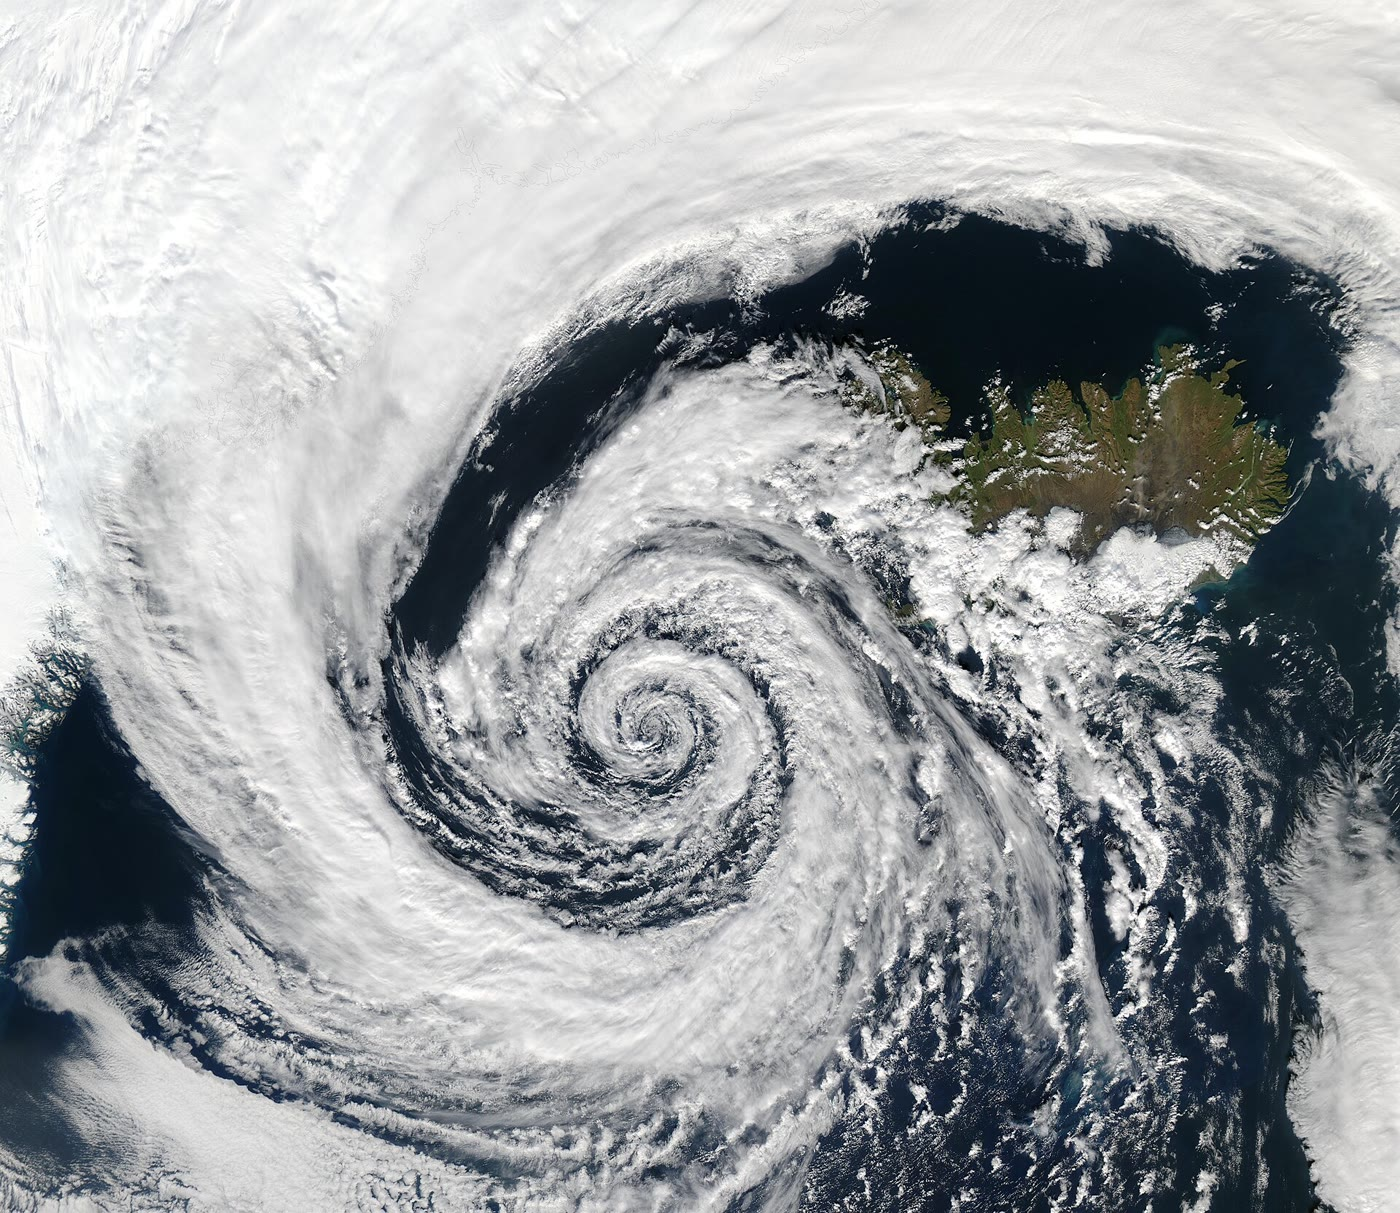
\includegraphics[width=\linewidth]{images/book1/g8-iceland-low.jpg}
\end{minipage}\hfill
\begin{minipage}[c]{0.6\linewidth}\raggedright
{\small Una \omterm{def:g8:fronts-and-weather-maps:depression}{borrasca} al sudoeste de Islandia (la isla de arriba a la
derecha) vista por el satélite Aqua de la NASA el 4~de septiembre de 2003.
Sus \omterm{def:g4:clouds-rain-snow:cloud}{nubes} giran en espiral hacia el centro, en sentido contrario a las
agujas del reloj, como en toda \omterm{def:g8:fronts-and-weather-maps:depression}{borrasca} del \omterm{def:g3:continents-and-oceans:equator}{hemisferio norte}. NASA/GSFC,
MODIS Rapid Response Team, Jacques Descloitres (dominio público, vía
Wikimedia Commons).}
\end{minipage}
% ledger: commons:iceland-low, bom:highs-lows
\label{fig:g8:fronts-and-weather-maps:iceland}
\end{omfigure}

\section{Las isobaras y los mapas del tiempo}

Para ver las \omterm{def:g8:fronts-and-weather-maps:depression}{borrascas} y los \omterm{def:g8:fronts-and-weather-maps:depression}{anticiclones}, los meteorólogos dibujan \omterm{def:g2:drawing-to-map:map}{mapas}
de la presión. Cada estación mide su presión y la reduce al \omterm{def:g4:world-physical-map:altitude}{nivel del mar},
para poder comparar una estación de \omterm{def:g1:landscapes-around-us:landform}{montaña} con una de la \omterm{def:g1:landscapes-around-us:water}{costa}. Después se
trazan líneas que pasan por todos los lugares donde la presión es la misma.
% ledger: bom:isobars

\begin{definition}[Isobara]\label{def:g8:fronts-and-weather-maps:isobar}
Una \emph{isobara}\index{isobara} es una línea de un \omterm{def:g2:drawing-to-map:map}{mapa} que une lugares
donde la presión al \omterm{def:g4:world-physical-map:altitude}{nivel del mar} es la misma. Las isobaras se rotulan en
hectopascales y a menudo se dibujan cada \qty{4}{hPa}.
\end{definition}
% ledger: bom:isobars (the 4 hPa step is the one of this book's maps)

Alrededor de una \omterm{def:g8:fronts-and-weather-maps:depression}{borrasca}, las \omterm{def:g8:fronts-and-weather-maps:isobar}{isobaras} forman curvas cerradas, con la
presión más baja en el centro, marcado con una B; alrededor de un
\omterm{def:g8:fronts-and-weather-maps:depression}{anticiclón} forman curvas cerradas con la presión más alta en el centro,
marcado con una A. Donde las \omterm{def:g8:fronts-and-weather-maps:isobar}{isobaras} están muy juntas, la presión cambia
deprisa de un lugar a otro, y el viento es fuerte; donde están muy
separadas, el viento es flojo.
% ledger: bom:isobars

\begin{omfigure}
\begin{tikzpicture}
\begin{axis}[width=14cm, axis equal image, xmin=0, xmax=2400, ymin=0, ymax=1600,
  hide axis, clip=true, axis background/.style={fill=white}]
  \addplot[isobar] table {figdata/out/grade-8-weather_map-isobars.dat};
  \addplot[warm front] table {figdata/out/grade-8-weather_map-warm.dat};
  \addplot[cold front] table {figdata/out/grade-8-weather_map-cold.dat};
  \addplot[quiver={u=\thisrow{u}, v=\thisrow{v}}, -{Stealth[length=1.5mm]}, omMeth, line width=0.6pt]
    table[x=x, y=y] {figdata/out/grade-8-weather_map-winds.dat};
  \addplot[only marks, mark=none, nodes near coords, point meta=explicit symbolic,
    every node near coord/.style={anchor=center, font=\tiny, fill=white, inner sep=0.6pt}]
    table[x=x, y=y, meta=level] {figdata/out/grade-8-weather_map-labels.dat};
  \node[font=\Large\bfseries, omCold, fill=white, inner sep=1pt] at (axis cs:690,1010) {B};
  \node[font=\scriptsize, anchor=north, fill=white, inner sep=0.5pt] at (axis cs:690,968) {980};
  \node[font=\Large\bfseries, omWarm] at (axis cs:1950,520) {A};
  \node[font=\scriptsize, anchor=north] at (axis cs:1950,485) {1034};
  \addplot[only marks, mark=square*, mark size=2pt, black] table[x=x, y=y] {figdata/out/grade-8-weather_map-town.dat};
  \node[font=\footnotesize\bfseries, anchor=west, fill=white, inner sep=1pt] at (axis cs:870,380) {T};
  \fill[white] (axis cs:1930,1450) rectangle (axis cs:2290,1585);
  \draw[line width=1pt] (axis cs:1950,1480) -- (axis cs:2250,1480);
  \pgfplotsinvokeforeach{1950,2050,2150,2250}{\draw (axis cs:#1,1460) -- (axis cs:#1,1500);}
  \node[font=\scriptsize, anchor=south] at (axis cs:2100,1495) {300 km};
\end{axis}
\end{tikzpicture}

{\small Un \omterm{def:g2:drawing-to-map:map}{mapa} del \omterm{def:g1:watching-the-weather:weather}{tiempo} de un día imaginario en el \omterm{def:g3:continents-and-oceans:equator}{hemisferio norte},
calculado a partir de un modelo de la presión. \omterm{def:g8:fronts-and-weather-maps:isobar}{Isobaras} cada
\qty{4}{hPa}; la \omterm{def:g8:fronts-and-weather-maps:depression}{borrasca} B (\qty{980}{hPa}) lleva un \omterm{def:g8:fronts-and-weather-maps:front}{frente cálido} (en
rojo) y un \omterm{def:g8:fronts-and-weather-maps:front}{frente frío} (en azul); el \omterm{def:g8:fronts-and-weather-maps:depression}{anticiclón} A (\qty{1034}{hPa}) está al
este. Flechas verdes: el viento, más largas donde es más fuerte. T: la
ciudad del problema.}
% ledger: bom:isobars, bom:highs-lows, mo:fronts (figdata/grade-8/weather_map.py)
\label{fig:g8:fronts-and-weather-maps:map}
\end{omfigure}

\begin{method}[Leer un mapa del tiempo]
\begin{enumerate}
  \item Busca los centros: B para las \omterm{def:g8:fronts-and-weather-maps:depression}{borrascas}, A para los \omterm{def:g8:fronts-and-weather-maps:depression}{anticiclones},
        con sus presiones.
  \item Lee las \omterm{def:g8:fronts-and-weather-maps:isobar}{isobaras}: sus valores aumentan hacia A y disminuyen hacia
        B. Las \omterm{def:g8:fronts-and-weather-maps:isobar}{isobaras} juntas indican un viento fuerte.
  \item Busca la dirección del viento: en el \omterm{def:g3:continents-and-oceans:equator}{hemisferio norte} sopla casi a
        lo largo de las \omterm{def:g8:fronts-and-weather-maps:isobar}{isobaras}, con las bajas presiones a su izquierda,
        un poco desviado hacia la baja.
  \item Busca los \omterm{def:g8:fronts-and-weather-maps:front}{frentes} y el sentido en que avanzan (el lado de sus
        símbolos), y luego el aire a cada lado: ¿qué viene a continuación?
\end{enumerate}
\end{method}
% ledger: bom:isobars, bom:highs-lows, mo:fronts

\begin{example}[El tiempo en la ciudad T]
En el \omterm{def:g2:drawing-to-map:map}{mapa}, T está al sur del \omterm{def:g8:fronts-and-weather-maps:front}{frente cálido} y al este del \omterm{def:g8:fronts-and-weather-maps:front}{frente frío}: en
el aire cálido entre los dos \omterm{def:g8:fronts-and-weather-maps:front}{frentes}. El \omterm{def:g8:fronts-and-weather-maps:front}{frente cálido} ya ha pasado por
ella. Allí las \omterm{def:g8:fronts-and-weather-maps:isobar}{isobaras} van del sudoeste al nordeste, con la baja al
noroeste: el viento sopla del sudoeste, cálido y húmedo. El \omterm{def:g8:fronts-and-weather-maps:front}{frente frío}
llega por el oeste. Sus triángulos apuntan al este, hacia la ciudad: en
unas horas habrá un breve episodio de chubascos fuertes y rachas, después
el viento girará al oeste o al noroeste, el aire se volverá más fresco y el
cielo se despejará.
\end{example}
% ledger: ucar:cold-front (figdata/grade-8/weather_map.py: wind at T from 227 degrees)

Un barómetro da su propio aviso, incluso sin \omterm{def:g2:drawing-to-map:map}{mapa}. Supón que todo el \omterm{def:g2:drawing-to-map:map}{mapa}
de arriba se desplazara hacia el este, sin cambiar, a \qty{40}{km} por
hora, y que un barómetro registrador estuviera en una estación S, al este
de los \omterm{def:g8:fronts-and-weather-maps:front}{frentes}. A lo largo de dos días y medio trazaría el registro de
abajo.

\begin{omfigure}
\begin{tikzpicture}
\begin{axis}[width=0.86\linewidth, height=5.4cm, xmin=0, xmax=60, ymin=980, ymax=1040,
  xtick={0,12,...,60}, ytick={980,990,...,1040},
  xlabel={horas desde el comienzo del registro}, ylabel={presión (hPa)},
  axis x line=bottom, axis y line=left, axis line style={-},
  grid=major, grid style={black!10},
  tick label style={font=\scriptsize}, label style={font=\small}, clip=false]
  \draw[omWarm!80!black, dashed] (axis cs:26.28,980) -- (axis cs:26.28,1040);
  \draw[omCold!80!black, dashed] (axis cs:38.49,980) -- (axis cs:38.49,1040);
  \node[font=\scriptsize, omWarm!80!black, anchor=south, fill=white, inner sep=1pt] at (axis cs:26.28,1032) {frente cálido};
  \node[font=\scriptsize, omCold!80!black, anchor=south, fill=white, inner sep=1pt] at (axis cs:38.49,1032) {frente frío};
  \addplot[black!80, line width=1pt] table[x=hour, y=p_hPa] {figdata/out/grade-8-barogram-trace.dat};
  \node[font=\scriptsize, anchor=north west, align=left] at (axis cs:2,1028) {anticiclón:\\tiempo estable};
  \node[font=\scriptsize, anchor=west] at (axis cs:39.5,986) {mínimo};
\end{axis}
\end{tikzpicture}

{\small El registro de un barómetro en la estación S mientras el \omterm{def:g2:drawing-to-map:map}{mapa} de
arriba se desplaza hacia el este a \qty{40}{km} por hora (una situación
inventada, calculada a partir del campo de presión del \omterm{def:g2:drawing-to-map:map}{mapa}). Líneas
discontinuas: el paso del \omterm{def:g8:fronts-and-weather-maps:front}{frente cálido} y del \omterm{def:g8:fronts-and-weather-maps:front}{frente frío} por la estación.}
% ledger: (invented region: weather situation of figdata/grade-8/weather_map.py, record from figdata/grade-8/barogram.py)
\end{omfigure}

\begin{example}[Leer el registro de un barómetro]\label{ex:g8:fronts-and-weather-maps:barogram}
Durante las 8 primeras horas, la presión sube hasta unos \qty{1031}{hPa}:
el \omterm{def:g8:fronts-and-weather-maps:depression}{anticiclón} pasa sobre S, con \omterm{def:g1:watching-the-weather:weather}{tiempo} estable. Después baja durante 30
horas, unos \qty{45}{hPa}: se acerca la \omterm{def:g8:fronts-and-weather-maps:depression}{borrasca}. Baja más deprisa unas
horas antes de que pase el \omterm{def:g8:fronts-and-weather-maps:front}{frente cálido}, más despacio en el aire cálido
que viene detrás, y alcanza su mínimo, unos \qty{986}{hPa}, justo cuando
pasa el \omterm{def:g8:fronts-and-weather-maps:front}{frente frío}. Después sube: la \omterm{def:g8:fronts-and-weather-maps:depression}{borrasca} se aleja, y llega el aire
más fresco y más limpio que hay detrás del \omterm{def:g8:fronts-and-weather-maps:front}{frente frío}.
% ledger: (invented region: figdata/grade-8/barogram.py), bom:highs-lows
\end{example}

\section{Cómo se hace una previsión}

\begin{definition}[Previsión meteorológica]\label{def:g8:fronts-and-weather-maps:forecast}
Una \emph{previsión meteorológica}\index{prevision meteorologica@previsión meteorológica}
es una descripción del \omterm{def:g1:watching-the-weather:weather}{tiempo} que se espera en un lugar durante las
próximas horas o los próximos días, elaborada a partir de observaciones de
la atmósfera y de las leyes de la física.
\end{definition}
% ledger: mo:how-forecasts

Una previsión se hace en tres pasos. Primero, los servicios meteorológicos
de todo el mundo hacen millones de observaciones cada día: temperatura,
\omterm{def:g4:clouds-rain-snow:precipitation}{precipitación}, presión, viento y humedad, medidos en estaciones de tierra,
en el \omterm{def:g2:water-on-earth:ocean}{mar}, con globos sonda, con radares y desde satélites. Después, esas
observaciones se introducen en modelos informáticos: ordenadores muy
potentes calculan, paso a paso, cómo cambiará la atmósfera a partir de su
estado actual. Por último, los predictores leen los resultados, los
comparan con lo que saben de su región y redactan la previsión.
% ledger: mo:how-forecasts

\begin{history}[La primera previsión pública]
En 1854, un oficial de marina, Robert FitzRoy, fue puesto al \omterm{def:g8:fronts-and-weather-maps:front}{frente} de una
nueva oficina meteorológica en Londres. Cada mañana a las 9, unas
estaciones repartidas por las \omterm{def:g1:landscapes-around-us:water}{costas} medían el \omterm{def:g1:watching-the-weather:weather}{tiempo} y enviaban sus
lecturas a Londres por telégrafo, el invento más moderno de la época. En
1859, un temporal terrible, el del \emph{Royal Charter}, hundió muchos
barcos; FitzRoy creó entonces un servicio de avisos de temporal para los
marinos, que empezó en febrero de 1861. El 1~de agosto de 1861 fue más
lejos y publicó la primera \omterm{def:g8:fronts-and-weather-maps:forecast}{previsión meteorológica} pública en un
periódico, \emph{The Times}. Sus previsiones miraban uno o dos días hacia
delante y eran muy generales; fueron el comienzo de las previsiones que
leemos hoy.
\end{history}
% ledger: mo:fitzroy

Las previsiones han mejorado mucho. En las últimas décadas, los
meteorólogos han ganado alrededor de un día más de buena previsión cada
diez años: una previsión a cuatro días es hoy tan buena como lo era una
previsión a un día hace treinta años. Pero cuanto más lejos mira una
previsión, menos segura es, porque los pequeños errores de las
observaciones de partida crecen a medida que el ordenador avanza en el
tiempo.
% ledger: bauer:day-per-decade, mo:accuracy

\begin{inthefield}[Ver llegar un frente]
Un día en que la previsión anuncie un \omterm{def:g8:fronts-and-weather-maps:front}{frente}, mira el cielo cada pocas
horas y anota la hora, las \omterm{def:g4:clouds-rain-snow:cloud}{nubes}, el viento y la temperatura. Antes de un
\omterm{def:g8:fronts-and-weather-maps:front}{frente cálido}, ¿llegan primero las finas estrías de los \omterm{def:g4:clouds-rain-snow:cloud-families}{cirros}? Cuando pasa
un \omterm{def:g8:fronts-and-weather-maps:front}{frente frío}, ¿baja la temperatura y cambia el viento? Compara tus notas
con el \omterm{def:g2:drawing-to-map:map}{mapa} del \omterm{def:g1:watching-the-weather:weather}{tiempo} del día.
\end{inthefield}

\section{Ejercicios}

\begin{exercise}[$\star$]\label{exo:g8:fronts-and-weather-maps:1}
Da el significado de cada par de letras y di si la \omterm{def:g8:fronts-and-weather-maps:air-mass}{masa de aire} es cálida
o fría, húmeda o seca: (a) mT; (b) cP; (c) cT; (d) mP.
\end{exercise}

\begin{exercise}[$\star$]\label{exo:g8:fronts-and-weather-maps:2}
Une cada signo de un \omterm{def:g2:drawing-to-map:map}{mapa} del \omterm{def:g1:watching-the-weather:weather}{tiempo} con su significado: una línea azul con
triángulos; una línea roja con semicírculos; una línea que une lugares con
la misma presión; la letra A; la letra B.
\end{exercise}

\begin{exercise}[$\star$]\label{exo:g8:fronts-and-weather-maps:3}
¿Verdadero o falso? Corrige las frases falsas. (a) Los \omterm{def:g8:fronts-and-weather-maps:depression}{anticiclones} suelen
traer un \omterm{def:g1:watching-the-weather:weather}{tiempo} estable. (b) Las \omterm{def:g4:clouds-rain-snow:cloud}{nubes} de un \omterm{def:g8:fronts-and-weather-maps:front}{frente cálido} llegan después
del \omterm{def:g8:fronts-and-weather-maps:front}{frente}. (c) Las \omterm{def:g8:fronts-and-weather-maps:isobar}{isobaras} juntas indican un viento flojo. (d) El aire
frío es más denso que el aire cálido.
\end{exercise}

\begin{exercise}[$\star$]\label{exo:g8:fronts-and-weather-maps:4}
En el \omterm{def:g2:drawing-to-map:map}{mapa} del \omterm{def:g1:watching-the-weather:weather}{tiempo} de este capítulo: (a) ¿cuál es la presión en el
centro de la \omterm{def:g8:fronts-and-weather-maps:depression}{borrasca}? (b) ¿Y en el del \omterm{def:g8:fronts-and-weather-maps:depression}{anticiclón}? (c) ¿Cuántos
hectopascales separan dos \omterm{def:g8:fronts-and-weather-maps:isobar}{isobaras} vecinas? (d) ¿En cuántos hectopascales
se diferencia la presión entre los dos centros?
\end{exercise}

\begin{exercise}[$\star\star$]\label{exo:g8:fronts-and-weather-maps:5}
Ordena estos acontecimientos tal como ocurren cuando un \omterm{def:g8:fronts-and-weather-maps:front}{frente cálido} se
acerca y pasa: \omterm{def:g4:clouds-rain-snow:precipitation}{lluvia} continua; finas estrías de \omterm{def:g4:clouds-rain-snow:cloud-families}{cirros}; un velo gris de
altostratos; aire más cálido y más húmedo; las \omterm{def:g4:clouds-rain-snow:cloud}{nubes} bajan y se espesan.
\end{exercise}

\begin{exercise}[$\star\star$]\label{exo:g8:fronts-and-weather-maps:6}
Explica por qué las \omterm{def:g4:clouds-rain-snow:cloud}{nubes} de un \omterm{def:g8:fronts-and-weather-maps:front}{frente frío} tienen un gran desarrollo
vertical, mientras que las de un \omterm{def:g8:fronts-and-weather-maps:front}{frente cálido} se extienden en capas. Usa
las palabras \emph{cuña}, \emph{empinada}, \emph{pendiente suave}.
\end{exercise}

\begin{exercise}[$\star\star$]\label{exo:g8:fronts-and-weather-maps:7}
En el \omterm{def:g2:drawing-to-map:map}{mapa} del \omterm{def:g1:watching-the-weather:weather}{tiempo}: (a) ¿dónde es más fuerte el viento, cerca de B o
cerca de A? ¿Cómo lo sabes? (b) Al norte de B, ¿de qué dirección sopla el
viento? (c) ¿Y al sur de A? (d) ¿Gira el viento alrededor de B en el
sentido de las agujas del reloj o en sentido contrario?
\end{exercise}

\begin{exercise}[$\star\star$]\label{exo:g8:fronts-and-weather-maps:8}
Un barómetro de una ciudad marca \qty{1016}{hPa} a las 6:00,
\qty{1009}{hPa} a las 12:00 y \qty{1003}{hPa} a las 18:00. (a) ¿Cuánto
baja la presión en 12 horas? (b) ¿Qué se acerca a la ciudad, una \omterm{def:g8:fronts-and-weather-maps:depression}{borrasca} o
un \omterm{def:g8:fronts-and-weather-maps:depression}{anticiclón}? (c) ¿Qué \omterm{def:g1:watching-the-weather:weather}{tiempo} puede esperar la ciudad?
\end{exercise}

\begin{exercise}[$\star\star$]\label{exo:g8:fronts-and-weather-maps:9}
Un aire que ha permanecido una semana sobre el Sáhara se desplaza hacia el
norte sobre el \omterm{def:g2:water-on-earth:ocean}{mar} Mediterráneo. (a) Designa esta \omterm{def:g8:fronts-and-weather-maps:air-mass}{masa de aire} con sus dos
letras. (b) ¿Es cálida o fría, húmeda o seca, cuando sale? (c) ¿Qué podría
cambiar en su carácter al cruzar el \omterm{def:g2:water-on-earth:ocean}{mar}?
\end{exercise}

\begin{exercise}[$\star\star$]\label{exo:g8:fronts-and-weather-maps:10}
Una previsión a cuatro días es hoy tan buena como lo era una previsión a
un día hace treinta años. (a) ¿Cuántos días de buena previsión se han
ganado en treinta años? (b) ¿Cuántos son por cada diez años? (c) Si el
progreso siguiera igual, ¿dentro de cuántos años sería una previsión a
cinco días tan buena como la previsión a un día de hoy?
\end{exercise}

\begin{exercise}[$\star\star\star$]\label{exo:g8:fronts-and-weather-maps:11}
En el \omterm{def:g2:drawing-to-map:map}{mapa} del \omterm{def:g1:watching-the-weather:weather}{tiempo}, usa la barra de \omterm{def:g2:drawing-to-map:scale}{escala}. (a) ¿Cuántos kilómetros,
más o menos, separan el centro B del centro A? (b) Cerca de B, dos
\omterm{def:g8:fronts-and-weather-maps:isobar}{isobaras} vecinas están a unos \qty{80}{km} una de otra. ¿Cuántos
hectopascales cambia allí la presión en \qty{100}{km}? (c) Cerca de A, dos
\omterm{def:g8:fronts-and-weather-maps:isobar}{isobaras} vecinas están a unos \qty{140}{km}. La misma pregunta. (d) ¿Dónde
es más fuerte el viento? ¿Coinciden las flechas del \omterm{def:g2:drawing-to-map:map}{mapa}?
\end{exercise}

\begin{exercise}[$\star\star\star$]\label{exo:g8:fronts-and-weather-maps:12}
Un \omterm{def:g8:fronts-and-weather-maps:front}{frente frío} está a \qty{300}{km} al oeste de una ciudad y avanza hacia
el este a \qty{50}{km} por hora; un \omterm{def:g8:fronts-and-weather-maps:front}{frente cálido} está a \qty{200}{km} al
oeste de otra ciudad y avanza a la mitad de esa velocidad. (a) ¿Qué \omterm{def:g8:fronts-and-weather-maps:front}{frente}
llega antes a su ciudad, y con cuántas horas de adelanto? (b) Describe el
\omterm{def:g1:watching-the-weather:weather}{tiempo} que verá cada ciudad cuando pase su frente. (c) ¿Qué ciudad estará
más cálida una vez que haya pasado su frente?
\end{exercise}

\section{Problema: ¿se suspenderá el partido por la lluvia?}

\begin{problem}[{Problema de fin de semana --- se juega un partido de fútbol
a las 15:00 en la ciudad T del mapa del tiempo; el frente frío se acerca:
se mide su velocidad en dos mapas y se prevé la hora a la que llegará a la
ciudad}]
\label{pb:g8:fronts-and-weather-maps:1}
% ledger: ucar:cold-front (figdata/grade-8/weather_map.py; the front's speed and the length of the showers are exercise data)
A las 09:00, una joven meteoróloga mira el \omterm{def:g2:drawing-to-map:map}{mapa} del \omterm{def:g1:watching-the-weather:weather}{tiempo} de este
capítulo y después el \omterm{def:g2:drawing-to-map:map}{mapa} de abajo: muestra el \omterm{def:g8:fronts-and-weather-maps:front}{frente frío} cerca de la
ciudad a las 06:00 y a las 09:00, sobre una cuadrícula de cuadrados de
\qty{20}{km}.

\begin{center}
\begin{tikzpicture}
\begin{axis}[width=11cm, axis equal image, xmin=0, xmax=600, ymin=0, ymax=400,
  xtick={0,100,...,600}, ytick={0,100,...,400}, minor tick num=4,
  grid=both, minor grid style={black!10}, major grid style={black!25},
  tick label style={font=\scriptsize}, xlabel={distancia hacia el este (km)}, ylabel={distancia hacia el norte (km)},
  label style={font=\small}]
  \addplot[cold front, densely dashed, opacity=0.55] table[x expr=\thisrow{x}-363.2, y expr=\thisrow{y}-180] {figdata/out/grade-8-weather_map-seq-06.dat};
  \addplot[cold front] table[x expr=\thisrow{x}-363.2, y expr=\thisrow{y}-180] {figdata/out/grade-8-weather_map-seq-09.dat};
  \addplot[only marks, mark=square*, mark size=2.2pt, black] table[x expr=\thisrow{x}-363.2, y expr=\thisrow{y}-180] {figdata/out/grade-8-weather_map-town.dat};
  \node[font=\footnotesize\bfseries, anchor=south west, fill=white, inner sep=1pt] at (axis cs:485,205) {T};
  \node[font=\scriptsize, fill=white, inner sep=1pt] at (axis cs:140,360) {06:00};
  \node[font=\scriptsize, fill=white, inner sep=1pt] at (axis cs:262,360) {09:00};
\end{axis}
\end{tikzpicture}
\end{center}

\noindent\textbf{Parte I --- Leer el mapa.}\par\nopagebreak
\begin{enumerate}[beginpenalty=10000]
  \item En el \omterm{def:g2:drawing-to-map:map}{mapa} del \omterm{def:g1:watching-the-weather:weather}{tiempo} del capítulo, ¿está la ciudad en el aire
        cálido o en el aire frío? ¿Qué \omterm{def:g8:fronts-and-weather-maps:front}{frente} ha pasado ya por ella?
  \item ¿De qué dirección sopla el viento en la ciudad?
  \item ¿Hacia dónde avanza el \omterm{def:g8:fronts-and-weather-maps:front}{frente frío}? ¿Cómo lo sabes por sus
        símbolos?
  \item ¿Qué \omterm{def:g1:watching-the-weather:weather}{tiempo} traerá el \omterm{def:g8:fronts-and-weather-maps:front}{frente frío} cuando pase?
\end{enumerate}

\noindent\textbf{Parte II --- La velocidad del frente.}\par\nopagebreak
\begin{enumerate}[resume, beginpenalty=10000]
  \item En el \omterm{def:g2:drawing-to-map:map}{mapa} de arriba, a la altura de la ciudad, ¿a qué distancia
        hacia el este está el frente a las 06:00? ¿Y a las 09:00?
  \item ¿Cuántos kilómetros ha avanzado el \omterm{def:g8:fronts-and-weather-maps:front}{frente} en esas tres horas?
  \item ¿Cuál es su velocidad, en kilómetros por hora?
  \item A las 09:00, ¿cuántos kilómetros separan el \omterm{def:g8:fronts-and-weather-maps:front}{frente} de la ciudad?
\end{enumerate}

\noindent\textbf{Parte III --- La previsión.}\par\nopagebreak
\begin{enumerate}[resume, beginpenalty=10000]
  \item Si el \omterm{def:g8:fronts-and-weather-maps:front}{frente} mantiene la misma velocidad, ¿cuántas horas necesitará
        para llegar a la ciudad?
  \item ¿A qué hora llegará a la ciudad?
  \item Supón que los chubascos fuertes duran alrededor de una hora después
        del paso del \omterm{def:g8:fronts-and-weather-maps:front}{frente}. ¿Seguirá lloviendo a las 15:00?
  \item El \omterm{def:g8:fronts-and-weather-maps:front}{frente} podría frenar hasta \qty{30}{km} por hora. ¿Cuándo
        llegaría entonces a la ciudad? Escribe la previsión para el partido
        en una o dos frases, dando las dos horas posibles.
\end{enumerate}
\end{problem}
